\documentclass[conference]{IEEEtran}
\IEEEoverridecommandlockouts
\usepackage{cite}
\usepackage{amsmath,amssymb,amsfonts}
\usepackage{algorithmic}
\usepackage{graphicx}
\usepackage{textcomp}
\usepackage{xcolor}
\usepackage{xurl} % Permite saltos de línea automáticos e impecables en URLs largas
\usepackage{hyperref}
\usepackage{float}
\def\BibTeX{{\rm B\kern-.05em{\sc i\kern-.025em b}\kern-.08em
    T\kern-.1667em\lower.7ex\hbox{E}\kern-.125emX}}

\begin{document}

\title{SheetMusic: Plataforma para la Enseñanza Adaptativa de Teoría Musical mediante un Modelo que Integra un Grafo de Conocimiento y Deep Reinforcement Learning}

\author{
\IEEEauthorblockN{Vicente Alves}
\IEEEauthorblockA{
\textit{Escuela de Ingeniería Civil en Informática} \\
\textit{Universidad Austral de Chile}\\
Valdivia, Chile \\
vicente.alves@alumnos.uach.cl}
\and
\IEEEauthorblockN{Fernando Inzulza}
\IEEEauthorblockA{
\textit{Escuela de Ingeniería Civil en Informática} \\
\textit{Universidad Austral de Chile}\\
Valdivia, Chile \\
fernando.inzulza@alumnos.uach.cl}
\and
\IEEEauthorblockN{Luis Veas-Castillo}
\IEEEauthorblockA{
\textit{Instituto de Informática} \\
\textit{Universidad Austral de Chile}\\
Valdivia, Chile \\
luis.veasc@inf.uach.cl}
\and
\IEEEauthorblockN{Christian Lazo}
\IEEEauthorblockA{
\textit{Instituto de Informática} \\
\textit{Universidad Austral de Chile}\\
Valdivia, Chile \\
clazo@inf.uach.cl}
\and
\IEEEauthorblockN{Abel Mansilla}
\IEEEauthorblockA{
\textit{Facultad de Arquitectura y Artes}\\
\textit{Universidad Austral de Chile}\\
Valdivia, Chile\\
abel.mansilla@uach.cl}
\and
}

\maketitle

\begin{abstract}
La enseñanza de la teoría musical en el contexto escolar enfrenta importantes desafíos derivados de la reducción de la carga horaria, la discontinuidad curricular y la heterogeneidad en los conocimientos previos de los estudiantes. Aunque existen diversas plataformas digitales de apoyo al aprendizaje musical, estas presentan una limitada capacidad de adaptación pedagógica y carecen de mecanismos que representen explícitamente las relaciones de dependencia entre los contenidos de aprendizaje.

Este trabajo propone un \textbf{modelo de aprendizaje adaptativo} que integra un \textbf{Grafo de Conocimiento Dirigido Acíclico (DAG)} para representar las dependencias pedagógicas entre conceptos de teoría musical y un agente basado en \textbf{Deep Reinforcement Learning (DRL)}, implementado mediante el algoritmo \textit{Proximal Policy Optimization (PPO)}, encargado de recomendar dinámicamente la siguiente actividad de aprendizaje de acuerdo con el estado de conocimiento de cada estudiante. Para facilitar el entrenamiento del agente, el modelo combina una etapa inicial de \textit{Behavior Cloning}, basada en estrategias pedagógicas definidas sobre el DAG, con un proceso posterior de aprendizaje por refuerzo en un entorno de simulación.

El modelo fue implementado en \textbf{SheetMusic}, una plataforma web progresiva orientada al aprendizaje adaptativo de teoría musical y al seguimiento pedagógico de los estudiantes por parte de los docentes. La validación experimental consideró una prueba piloto de 28 días con 28 estudiantes y una evaluación de aceptación tecnológica con docentes de la Región de Los Ríos, Chile.

Los resultados muestran una mejora aproximada del \textbf{20\%} en la mediana del nivel de \textit{proficiency} de los estudiantes, acompañada de una alta percepción de usabilidad (\textbf{SUS = 82.5/100}) y una positiva aceptación tecnológica por parte de los docentes (\textbf{TAM = 3.75/5} en utilidad percibida y \textbf{4.00/5} en facilidad de uso). En conjunto, estos resultados evidencian que la integración de un grafo de conocimiento con \textbf{Deep Reinforcement Learning} constituye una estrategia viable para desarrollar sistemas de aprendizaje adaptativo en el dominio de la teoría musical.


%La educación musical escolar enfrenta severos desafíos derivados de la reducción de la carga horaria, la falta de linealidad curricular y la alta heterogeneidad en los conocimientos de los estudiantes. Las herramientas digitales existentes carecen de alineación curricular local, flexibilidad adaptativa y mecanismos de gestión pedagógica para el cuerpo docente. Este trabajo presenta el diseño, implementación y validación de SheetMusic, una plataforma web progresiva y servicio web distribuido para la enseñanza adaptativa de la teoría musical. El sistema articula la experiencia de aprendizaje del estudiante mediante un grafo de conocimiento no lineal y gamificado, herramientas de seguimiento pedagógico para el docente, y un microservicio inteligente basado en Aprendizaje por Refuerzo Profundo (DRL) mediante el algoritmo Proximal Policy Optimization (PPO) que ajusta en tiempo real la dificultad de las actividades. El conocimiento musical se formalizó en un Grafo Dirigido Acíclico (DAG) de 23 nodos que modela las dependencias pedagógicas. La validación experimental abarcó pruebas piloto durante 28 días con 28 estudiantes y un estudio cuali-cuantitativo (entrevistas y pruebas de usabilidad) con 6 docentes de la Región de Los Ríos, Chile. Los resultados demostraron una mejora en la mediana de desempeño (proficiency) del 20\% impulsada por el motor DRL, una alta usabilidad percibida por parte de los estudiantes (SUS de 82.5/100) y una positiva aceptación tecnológica docente (TAM con 3.75/5 en utilidad percibida y 4.00/5 en facilidad de uso).
\end{abstract}

\begin{IEEEkeywords}
Aprendizaje Adaptativo, Deep Reinforcement Learning, Grafo de Conocimiento, Recomendación Adaptativa, Teoría Musical, Sistemas Inteligentes Educativos.
%Aprendizaje Adaptativo, Educación Musical, Servicio Web, Deep Reinforcement Learning, Grafos de Conocimiento, Usabilidad, TAM.
\end{IEEEkeywords}
\section{INTRODUCCIÓN}

La formación musical escolar desempeña un rol fundamental en el desarrollo cognitivo, creativo y crítico de los estudiantes. Sin embargo, durante las últimas décadas la enseñanza de la música en Chile ha experimentado una progresiva reducción de su presencia dentro del currículo escolar. Decretos ministeriales como el N.\textsuperscript{o} 2960 y el N.\textsuperscript{o} 628 disminuyen la carga horaria destinada a la asignatura a medida que los estudiantes avanzan en su trayectoria escolar, obligando a compartir horas con Artes Visuales o relegando la música a un plan electivo en los niveles superiores~\cite{mineduc_decreto2960_2012, mineduc_decreto628_2016}.

Esta disminución de la carga horaria ha generado dos problemas relevantes para el proceso de enseñanza-aprendizaje de la teoría musical:

\begin{enumerate}
\item \textbf{Discontinuidad curricular y heterogeneidad del aprendizaje.} La reducción de horas y la falta de continuidad en los programas provocan que los estudiantes lleguen a cursos superiores con importantes diferencias en sus conocimientos musicales, dificultando el trabajo del docente y el desarrollo de actividades homogéneas dentro del aula~\cite{chandia_educacion_2025}.

\item \textbf{Limitada disponibilidad de herramientas adaptativas para el contexto escolar.} Aunque existen plataformas digitales orientadas al aprendizaje musical, como Yousician o Simply Piano, estas han sido diseñadas principalmente para contextos de autoaprendizaje, presentan escasa alineación con el currículo escolar chileno y utilizan rutas de aprendizaje predominantemente lineales, sin considerar explícitamente las dependencias pedagógicas entre los contenidos ni las necesidades particulares de cada estudiante~\cite{garcia2025, alrowais2025, li2025}.
\end{enumerate}

Como consecuencia, los docentes deben enfrentar cursos con niveles de conocimiento altamente heterogéneos, mientras que las herramientas tecnológicas disponibles ofrecen una capacidad limitada para adaptar dinámicamente las actividades de aprendizaje según el progreso individual de cada estudiante. Esta situación evidencia la necesidad de modelos computacionales capaces de representar explícitamente la estructura del dominio de conocimiento y utilizar dicha representación para personalizar el proceso de enseñanza.

En este contexto surge la siguiente pregunta de investigación:

\begin{quote}
\textit{¿Cómo desarrollar un modelo computacional de aprendizaje adaptativo capaz de recomendar dinámicamente actividades de teoría musical de acuerdo con el progreso del estudiante y la estructura pedagógica del dominio?}
\end{quote}

Se plantea como hipótesis que la integración de una representación explícita del conocimiento pedagógico con un modelo basado en \textit{Deep Reinforcement Learning} (DRL), capaz de aprender políticas de decisión adaptativas a partir de la interacción con el entorno~\cite{sutton2018reinforcement,mnih2015human}, permite generar recomendaciones personalizadas que mejoran el proceso de aprendizaje de teoría musical, ajustando dinámicamente la secuencia de actividades de acuerdo con el progreso individual del estudiante y las dependencias existentes entre los contenidos.

Para validar esta hipótesis se desarrolló \textbf{SheetMusic}, una plataforma para la enseñanza adaptativa de teoría musical que implementa el modelo propuesto mediante la integración de un Grafo de Conocimiento Dirigido Acíclico (DAG), utilizado para representar las relaciones de dependencia entre los contenidos musicales, y un agente basado en \textit{Deep Reinforcement Learning}, encargado de recomendar dinámicamente la siguiente actividad de aprendizaje para cada estudiante. La plataforma incorpora además herramientas de seguimiento pedagógico que permiten al docente monitorear el progreso individual de sus estudiantes.

Las principales contribuciones de este trabajo son las siguientes:

\begin{itemize}
\item La formalización del dominio de teoría musical mediante un Grafo de Conocimiento Dirigido Acíclico que representa explícitamente las dependencias pedagógicas entre los contenidos.

\item El desarrollo de un modelo de aprendizaje adaptativo basado en \textit{Deep Reinforcement Learning}, capaz de recomendar dinámicamente actividades de acuerdo con el estado de aprendizaje de cada estudiante.

\item La implementación del modelo en la plataforma \textbf{SheetMusic}, integrando el motor inteligente dentro de una arquitectura distribuida orientada al aprendizaje adaptativo.

\item La validación experimental del modelo mediante una prueba piloto realizada con estudiantes y docentes de la Región de Los Ríos, evaluando tanto el desempeño del modelo adaptativo como la percepción de usabilidad y aceptación tecnológica de la plataforma.
\end{itemize}

El resto del artículo se organiza de la siguiente manera. La Sección II presenta los trabajos relacionados y el estado del arte. La Sección III describe el modelo propuesto y la arquitectura de la plataforma \textbf{SheetMusic}. La Sección IV presenta la validación experimental y los resultados obtenidos. Finalmente, la Sección V expone las conclusiones y las principales líneas de trabajo futuro.
\section{TRABAJOS RELACIONADOS Y ESTADO DEL ARTE}

El aprendizaje adaptativo de teoría musical constituye un área interdisciplinaria donde convergen la educación musical, la inteligencia artificial y los sistemas inteligentes de apoyo al aprendizaje. En esta sección se revisan las principales plataformas existentes, los avances recientes en representación del conocimiento y aprendizaje adaptativo, y la brecha científica que motiva el presente trabajo.

\subsection{Plataformas de Aprendizaje Musical}

En el ámbito comercial y de acceso abierto destacan plataformas como \textit{Yousician}, \textit{Simply Piano}, \textit{Teoria.com} y \textit{Duolingo Music}. Estas herramientas han contribuido significativamente a masificar el acceso al aprendizaje musical mediante experiencias gamificadas e interfaces interactivas. Sin embargo, presentan diversas limitaciones para su incorporación como herramientas de apoyo en el contexto escolar:

\begin{itemize}

\item \textbf{Alineación curricular e idioma:} La mayoría de estas plataformas fueron desarrolladas para mercados angloparlantes y no se encuentran alineadas con las bases curriculares del sistema educativo chileno ni latinoamericano~\cite{garcia2025,alrowais2025}.

\item \textbf{Apoyo al proceso docente:} Su diseño está orientado principalmente al autoaprendizaje, careciendo de mecanismos que permitan al profesor monitorear el progreso de los estudiantes, identificar brechas de aprendizaje o asignar actividades diferenciadas~\cite{garcia2025,alrowais2025,li2025}.

\item \textbf{Secuencias de aprendizaje rígidas:} Generalmente organizan los contenidos mediante rutas de aprendizaje predefinidas o predominantemente lineales, limitando la personalización del recorrido formativo y la incorporación de representaciones explícitas de las dependencias pedagógicas entre los contenidos~\cite{alrowais2025,li2025}.

\end{itemize}

\subsection{Representación del Conocimiento y Aprendizaje Adaptativo}

La representación explícita del dominio de conocimiento constituye un componente fundamental en los sistemas de aprendizaje adaptativo, ya que permite modelar las relaciones de dependencia entre conceptos, definir prerrequisitos y estructurar trayectorias de aprendizaje coherentes~\cite{manrique2019kg}. En el dominio de la teoría musical, esta representación resulta especialmente relevante debido a la naturaleza progresiva de los contenidos, donde la comprensión de conceptos avanzados depende del dominio previo de conocimientos fundamentales.

Paralelamente, la incorporación de técnicas de Inteligencia Artificial en educación ha experimentado un importante crecimiento durante los últimos años. En el ámbito de la educación musical, diversos trabajos han explorado el uso de IA para la generación automática de contenidos, entrenamiento auditivo y evaluación del desempeño de los estudiantes~\cite{garcia2025}.

Particularmente, el \textit{Deep Reinforcement Learning} (DRL) ha demostrado ser una alternativa efectiva para resolver problemas de decisión secuencial y personalización del aprendizaje, permitiendo aprender políticas de recomendación adaptativas a partir de la interacción con el entorno~\cite{sutton2018reinforcement,mnih2015human}. Entre los algoritmos más utilizados destacan \textit{Deep Q-Network} (DQN) y \textit{Proximal Policy Optimization} (PPO), ampliamente empleados para el aprendizaje de políticas en problemas de decisión secuencial. En educación, estos enfoques han sido utilizados para optimizar trayectorias de aprendizaje considerando el desempeño y la evolución individual de cada estudiante~\cite{alrowais2025,li2025}.

No obstante, en el dominio de la educación musical la mayor parte de las investigaciones se han concentrado en composición asistida por IA, entrenamiento auditivo o herramientas de apoyo institucional. Asimismo, las investigaciones revisadas no consideran simultáneamente una representación explícita del conocimiento disciplinar y un mecanismo de decisión basado en aprendizaje por refuerzo para recomendar trayectorias de aprendizaje adaptativas.

\subsection{Brecha Científica}

Del análisis del estado del arte se observa que las soluciones existentes abordan parcialmente el problema del aprendizaje adaptativo. Mientras las plataformas comerciales proporcionan experiencias de aprendizaje gamificadas, los trabajos de investigación exploran la utilización de técnicas de inteligencia artificial para personalizar el proceso educativo. Sin embargo, no se identifican propuestas que integren simultáneamente:

\begin{enumerate}

\item Una representación explícita del conocimiento de teoría musical que modele las dependencias pedagógicas entre los contenidos.

\item Un modelo basado en \textit{Deep Reinforcement Learning} capaz de recomendar dinámicamente la siguiente actividad de aprendizaje de acuerdo con el progreso del estudiante.

\item Una plataforma que permita implementar dicho modelo en un entorno real, incorporando además herramientas de seguimiento pedagógico para el docente.

\end{enumerate}

Esta brecha evidencia la necesidad de desarrollar modelos computacionales que integren una representación explícita del conocimiento con técnicas de aprendizaje adaptativo, permitiendo recomendar dinámicamente actividades de teoría musical de acuerdo con el progreso individual del estudiante y la estructura pedagógica del dominio.
\section{SOLUCIÓN PROPUESTA}

La solución propuesta consiste en un modelo computacional de aprendizaje adaptativo para la enseñanza de teoría musical, diseñado para recomendar dinámicamente actividades de acuerdo con el progreso individual del estudiante y la estructura pedagógica del dominio. El modelo se estructura sobre tres componentes complementarios: (i) un Grafo de Conocimiento Dirigido Acíclico (DAG), encargado de representar explícitamente las dependencias entre los conceptos musicales; (ii) un agente basado en \textit{Deep Reinforcement Learning} (DRL), responsable de aprender una política de recomendación adaptativa; y (iii) la plataforma \textbf{SheetMusic}, que implementa el modelo y proporciona las funcionalidades necesarias para estudiantes y docentes.

El modelo fue implementado en \textbf{SheetMusic}, una plataforma web progresiva que articula la experiencia de aprendizaje del estudiante, las herramientas de seguimiento pedagógico del docente y un microservicio inteligente encargado de generar las recomendaciones. La separación entre la representación del conocimiento, el motor de decisión y la plataforma permite desacoplar la lógica adaptativa de los componentes de presentación, persistencia y procesamiento inteligente.

%--------------------------------------------------------
\subsection{Modelo Funcional de SheetMusic}

La implementación del modelo de aprendizaje adaptativo se materializa mediante \textbf{SheetMusic}, una plataforma web progresiva diseñada para apoyar tanto el proceso de aprendizaje de los estudiantes como el seguimiento pedagógico realizado por los docentes. Desde una perspectiva funcional, la plataforma define dos actores principales: el \textit{Estudiante}, quien interactúa con el sistema mediante actividades de estudio, práctica y seguimiento de su progreso; y el \textit{Profesor}, responsable de la gestión de cursos, la administración de estudiantes, la asignación de actividades y el monitoreo del desempeño académico.

La Figura~\ref{fig:casos_uso} presenta la visión funcional de SheetMusic mediante un diagrama de casos de uso unificado, mostrando las principales funcionalidades disponibles para ambos perfiles de usuario. Esta visión funcional establece el contexto operativo sobre el cual se implementa el modelo computacional de aprendizaje adaptativo descrito en las siguientes subsecciones.

\begin{figure}[htbp]
    \centering
    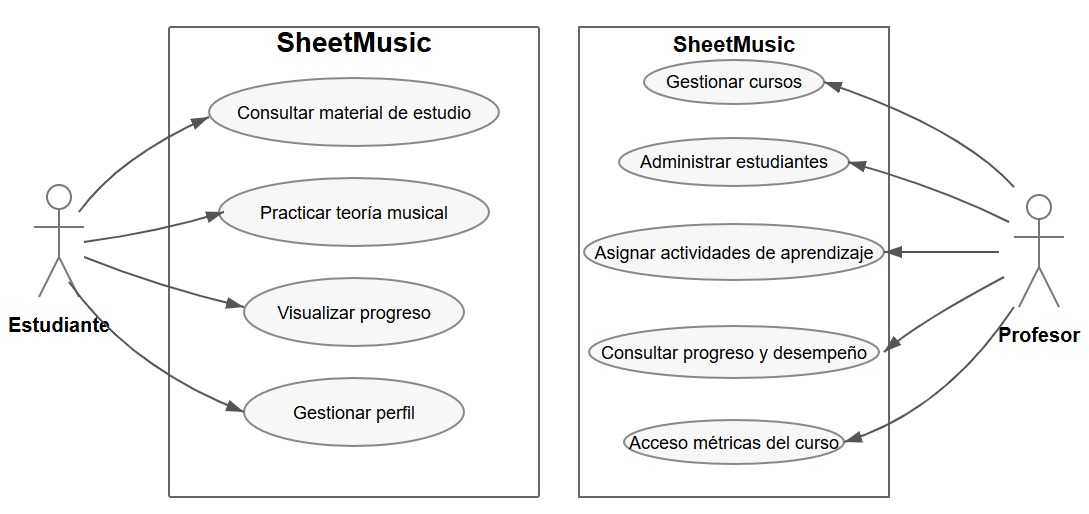
\includegraphics[width=0.3\textwidth]{Imagenes/caso_uso.jpeg}
    \caption{Modelo funcional de la plataforma SheetMusic, mostrando los principales casos de uso para los perfiles de Estudiante y Profesor.}
    \label{fig:casos_uso}
\end{figure}

%--------------------------------------------------------
\subsection{Grafo de Conocimiento Musical}

La representación explícita del dominio de conocimiento constituye uno de los pilares del modelo de aprendizaje adaptativo propuesto, ya que permite formalizar computacionalmente las relaciones pedagógicas existentes entre los distintos contenidos de teoría musical. En lugar de organizar los ejercicios mediante una secuencia fija, el modelo representa el dominio como una estructura de dependencias que permite identificar prerrequisitos, establecer trayectorias de aprendizaje coherentes y restringir las recomendaciones a actividades pedagógicamente válidas~\cite{manrique2019kg}.

Con este propósito, el dominio de la teoría musical se formalizó mediante un \textbf{Grafo de Conocimiento Dirigido Acíclico (DAG)} definido como:

\begin{equation}
G=(V,E)
\end{equation}

donde $V$ representa el conjunto de unidades de conocimiento (nodos) y $E$ el conjunto de aristas dirigidas que modelan las relaciones de dependencia pedagógica entre dichos conceptos. En la implementación completa del sistema, el grafo está compuesto por 23 unidades de conocimiento distribuidas en cinco niveles de dificultad y 29 relaciones de dependencia. Estas dependencias representan prerrequisitos recomendados para favorecer una progresión lógica del aprendizaje, aunque no constituyen restricciones absolutas, ya que un estudiante puede acceder a contenidos posteriores cuando demuestra un nivel de dominio suficiente durante el proceso de evaluación adaptativa.

Con el propósito de facilitar la validación experimental del modelo, en este trabajo se empleó un subgrafo compuesto por cuatro unidades de conocimiento fundamentales de teoría musical: \textit{Notas y Ritmo}, \textit{Intervalos}, \textit{Escalas Mayores y Menores} y \textit{Acordes (Tríadas)}. Estos conceptos permiten representar las principales relaciones de dependencia pedagógica presentes en el dominio y constituyen una base suficiente para evaluar el comportamiento del sistema de recomendación.

\begin{figure}[htbp]
    \centering
    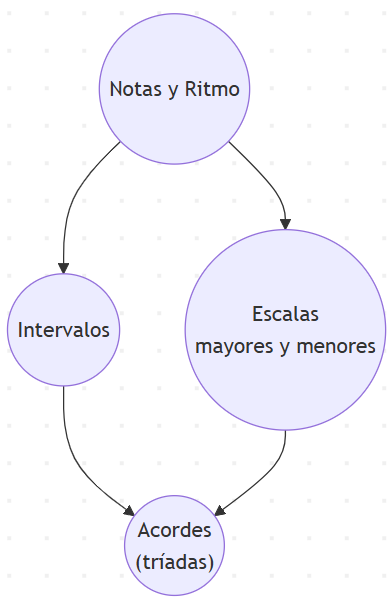
\includegraphics[width=0.15\textwidth]{Imagenes/grafo_dag.png}
    \caption{Subgrafo del Grafo de Conocimiento Musical utilizado durante la validación experimental. Cada nodo representa una unidad de conocimiento y cada arista dirigida representa una relación de prerrequisito pedagógico entre conceptos.}
    \label{fig:dag}
\end{figure}

La Figura~\ref{fig:dag} muestra el subgrafo utilizado durante la validación. En esta representación, las aristas dirigidas indican los prerrequisitos pedagógicos entre los distintos conceptos, permitiendo establecer una progresión lógica del aprendizaje desde contenidos básicos hacia unidades de mayor complejidad.

Para que el agente de recomendación pueda determinar las actividades disponibles en cada instante del proceso de aprendizaje, cada nodo del grafo mantiene un estado asociado al progreso alcanzado por el estudiante. Dicho estado puede corresponder a una unidad bloqueada (\textit{locked}), disponible (\textit{available}), en desarrollo (\textit{active}) o completada (\textit{done}), según la siguiente definición:

\begin{equation}
State(v_i)=
\begin{cases}
\text{locked}, & \exists u \in Pred(v_i)\mid Prog(u)\neq\text{done}\\
\text{done}, & Prog(v_i)=\text{done}\\
\text{active}, & Prog(v_i)=\text{in\_progress}\\
\text{available}, & \text{en otro caso}
\end{cases}
\end{equation}

Esta representación no determina directamente cuál será la siguiente actividad recomendada, sino que define el conjunto de actividades pedagógicamente válidas para el estado actual del estudiante. Sobre este espacio de decisión opera posteriormente el agente basado en \textit{Deep Reinforcement Learning}, encargado de seleccionar la recomendación que maximiza el progreso esperado del proceso de aprendizaje.

%--------------------------------------------------------
\subsection{Modelo de Recomendación Basado en Deep Reinforcement Learning}

Una vez representado el dominio de conocimiento mediante el Grafo de Conocimiento Musical, el problema de recomendación adaptativa se modela como un proceso de decisión secuencial, donde un agente basado en \textit{Deep Reinforcement Learning} (DRL) selecciona dinámicamente la siguiente actividad de aprendizaje considerando el estado actual del estudiante y las restricciones pedagógicas definidas por el DAG. El objetivo del agente consiste en aprender una política de recomendación que maximice el progreso esperado del estudiante, equilibrando la consolidación de conocimientos, la exploración de nuevos contenidos y la dificultad de los ejercicios.

La implementación del agente se desarrolló utilizando \textit{Stable-Baselines3} (versión 2.0.1) sobre \textit{Gymnasium} (versión 1.2.0), siguiendo el esquema clásico de interacción \textit{agent-environment loop}, donde el agente observa el estado del estudiante, selecciona una actividad, recibe retroalimentación y actualiza iterativamente su política de decisión.

\subsubsection{Entorno de Aprendizaje}

El entorno de entrenamiento, denominado \texttt{MusicLearningEnv}, fue implementado como una subclase de \texttt{gymnasium.Env}. Cada interacción corresponde a un episodio donde el agente selecciona un ejercicio de teoría musical, observa la respuesta del estudiante y recibe una recompensa asociada al impacto pedagógico de dicha decisión.

\subsubsection{Espacio de Observaciones}

El estado del estudiante se representa mediante la clase \texttt{UserState}, la cual encapsula la información necesaria para describir su situación de aprendizaje. Entre los atributos considerados se encuentran: \textbf{knowledge} (nivel de dominio de cada concepto), \textbf{accuracy} (precisión histórica), \textbf{attempts} (cantidad de intentos por concepto), \textbf{streak} (racha de aciertos o errores), \textbf{last\_exercise\_difficulty} (última dificultad presentada), \textbf{time\_since\_last\_practice} (tiempo desde la última práctica) y \textbf{recent\_performance\_trend} (tendencia reciente de desempeño).

Para el proceso de inferencia, el nivel de dominio se discretiza utilizando un umbral de proficiencia de 0.5:

\begin{equation}
o_i=
\begin{cases}
1, & \text{si } proficiency_i \ge 0.5\\
0, & \text{en otro caso}
\end{cases}
\end{equation}

obteniéndose un vector binario (\texttt{MultiBinary}) que resume el estado de conocimiento del estudiante y constituye la entrada utilizada por el agente DRL.

\subsubsection{Espacio de Acciones}

El espacio de acciones se define como un conjunto discreto (\texttt{Discrete(N)}), donde cada acción corresponde a un ejercicio específico de teoría musical asociado a uno de los nodos del DAG mediante la estructura \texttt{skill\_mapping}. Esta representación desacopla el modelo de aprendizaje del conjunto de ejercicios disponible, permitiendo incorporar nuevos contenidos o eliminar ejercicios existentes sin modificar la estructura del agente.

\subsubsection{Función de Recompensa}

La política del agente se aprende mediante la maximización de una recompensa acumulada que refleja el equilibrio entre el progreso pedagógico del estudiante y la calidad de las recomendaciones generadas. Para ello, se definió una función de recompensa compuesta por incentivos y penalizaciones, orientada a favorecer trayectorias de aprendizaje efectivas y evitar decisiones pedagógicamente inadecuadas.

\begin{equation}
\begin{aligned}
R =\;&
1.0\,\mathbb{I}(\text{correcto})
+0.5\,\mathbb{I}(\text{mejoría}) \\
&+0.5\,\mathbb{I}\!\left(
|d-d^{*}|\le1
\right)
-0.3\,\mathbb{I}\!\left(
|d-d^{*}|>2
\right) \\
&+0.2\,\mathbb{I}(\text{nodo poco practicado})
+0.1\,\mathbb{I}(\text{ejercicio nuevo})
\end{aligned}
\end{equation}

donde $d^{*}=proficiency\times10$ representa la dificultad esperada para el nivel actual del estudiante.

Los términos positivos incentivan respuestas correctas, mejoras respecto al desempeño previo, ejercicios cercanos a la zona de desarrollo proximal, exploración de contenidos poco practicados y variedad en las actividades recomendadas. Por otra parte, el agente recibe penalizaciones cuando recomienda ejercicios cuya dificultad resulta inadecuada para el nivel del estudiante, cuando repite innecesariamente un mismo ejercicio o cuando intenta acceder a contenidos cuyos prerrequisitos pedagógicos definidos por el DAG aún no han sido alcanzados. En consecuencia, el agente aprende simultáneamente a maximizar el progreso esperado del estudiante y a minimizar recomendaciones pedagógicamente inconsistentes.

\subsubsection{Selección del Algoritmo de Aprendizaje}

Con el objetivo de determinar el algoritmo más adecuado para el problema de recomendación adaptativa, se evaluaron dos enfoques ampliamente utilizados en Deep Reinforcement Learning: \textit{Deep Q-Network} (DQN) y \textit{Proximal Policy Optimization} (PPO).

Durante las pruebas experimentales, DQN presentó una convergencia inicial más rápida, alcanzando políticas aceptables después de aproximadamente 120 episodios. Sin embargo, mostró una tendencia a favorecer acciones previamente exitosas, reduciendo la exploración de nuevos contenidos y generando políticas excesivamente conservadoras.

Por el contrario, PPO presentó una convergencia ligeramente más lenta (150--180 episodios), pero desarrolló políticas considerablemente más estables, manteniendo un mejor equilibrio entre exploración y explotación. Además, su arquitectura \textit{actor-critic} y el uso de políticas estocásticas permitieron obtener recomendaciones menos predecibles y más consistentes con la variabilidad esperada en procesos educativos adaptativos. Por estas razones, PPO fue seleccionado como algoritmo de recomendación del sistema.

\subsubsection{Estrategia de Entrenamiento}

Debido a que durante las primeras etapas del proyecto no se disponía de datos históricos de interacción suficientes para entrenar el agente mediante aprendizaje por refuerzo, se diseñó una estrategia de entrenamiento en dos etapas.

En primer lugar, se aplicó un cuestionario a estudiantes de enseñanza media para estimar perfiles iniciales de conocimiento y parámetros de aprendizaje. A partir de estos datos se implementó un simulador probabilístico denominado \texttt{SyntheticStudent}, capaz de generar trayectorias sintéticas de aprendizaje para distintos perfiles de estudiantes.

Posteriormente, el entrenamiento se realizó mediante un esquema híbrido. Inicialmente se aplicó \textit{Behavior Cloning}, técnica de aprendizaje por imitación utilizada para inicializar una política a partir de demostraciones o decisiones de referencia~\cite{osa2018imitation}. En este trabajo, dicha política inicial fue construida utilizando criterios pedagógicos definidos por expertos en teoría musical. Sobre esta política base se ejecutó posteriormente el entrenamiento mediante PPO utilizando aproximadamente 200\,000 interacciones simuladas, permitiendo refinar progresivamente la política de recomendación hasta obtener un comportamiento estable y adaptativo.

Este enfoque híbrido combina conocimiento pedagógico explícito, incorporado inicialmente mediante \textit{Behavior Cloning}, con la capacidad de optimización autónoma proporcionada por \textit{Deep Reinforcement Learning}. Como resultado, el agente inicia el proceso de aprendizaje a partir de una política consistente con criterios pedagógicos definidos por expertos y posteriormente la refina mediante interacción con el entorno, obteniendo recomendaciones progresivamente más adaptativas y robustas.

%--------------------------------------------------------
\subsection{Arquitectura Distribuida}

La implementación del modelo de aprendizaje adaptativo propuesto se materializa mediante una arquitectura distribuida basada en microservicios, diseñada para desacoplar la interfaz de usuario, la gestión de datos y el motor de inteligencia artificial encargado de generar las recomendaciones adaptativas. Esta separación permite que cada componente evolucione de manera independiente, facilita el escalamiento horizontal del sistema y posibilita incorporar mejoras al modelo de aprendizaje sin modificar la plataforma utilizada por estudiantes y docentes \cite{charland_mobile_2011,flutter_vs_ionic_2023}.

La Figura~\ref{fig:arquitectura} presenta la arquitectura general de \textbf{SheetMusic}, organizada en tres capas principales: una capa cliente responsable de la interacción con los usuarios, una capa de servicios encargada de la autenticación y persistencia de la información académica, y una capa de inteligencia donde se ejecuta el modelo basado en \textit{Deep Reinforcement Learning}.

%--------------------------------------------------------
% FIGURA 3
% Arquitectura General
%--------------------------------------------------------

\begin{figure}[htbp]
    \centering
    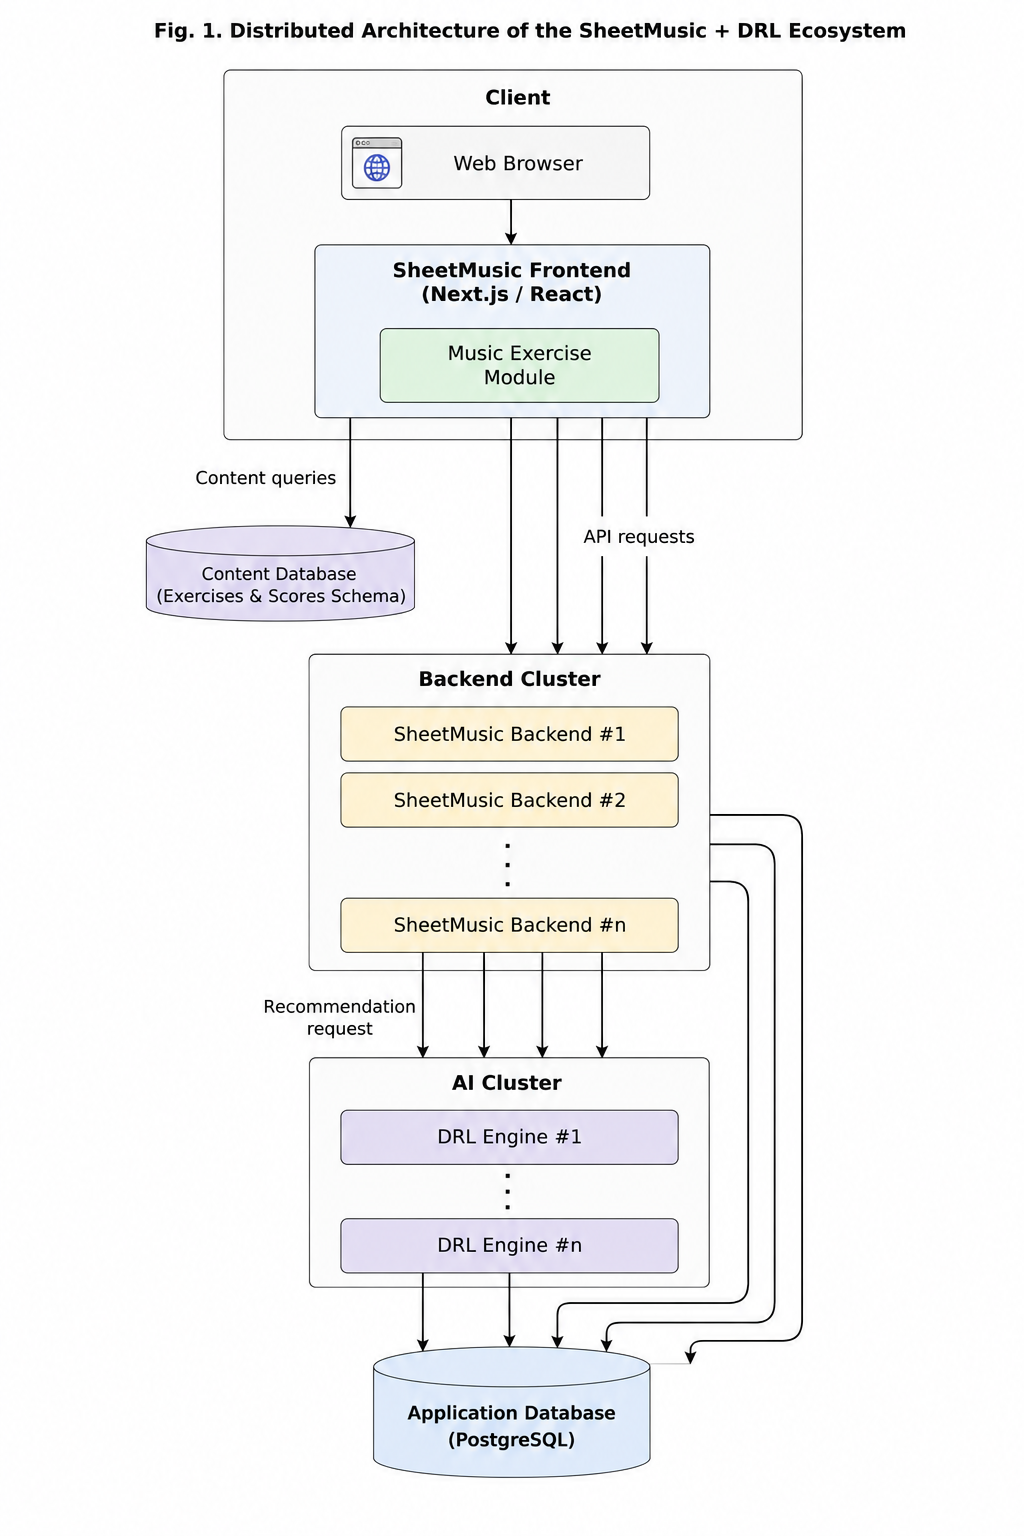
\includegraphics[width=0.3\textwidth]{Imagenes/fig_arch_system.png}
    \caption{Arquitectura distribuida de SheetMusic y sus principales componentes.}
    \label{fig:arquitectura}
\end{figure}

\subsubsection{Componentes de la Arquitectura}

La arquitectura propuesta está compuesta por tres componentes principales:

\begin{itemize}

\item \textbf{Capa Cliente.} Implementada como una \textit{Progressive Web Application} (PWA) utilizando Ionic React y Capacitor, proporciona la interfaz mediante la cual estudiantes y docentes acceden al material de estudio, resuelven ejercicios, consultan su progreso académico y administran las actividades del curso.

\item \textbf{Capa de Servicios.} Implementada sobre Supabase y PostgreSQL, administra la autenticación de usuarios mediante \textit{JSON Web Tokens} (JWT), el almacenamiento del historial académico y la comunicación con la aplicación cliente mediante procedimientos remotos (RPC). Asimismo, aplica políticas de seguridad basadas en \textit{Row Level Security} (RLS), garantizando el aislamiento de la información entre estudiantes y docentes \cite{supabase_docs_2024}.

\item \textbf{Motor de Inteligencia.} Implementado como un microservicio independiente utilizando FastAPI, PyTorch y Stable-Baselines3, recibe el estado actualizado del estudiante, ejecuta el agente basado en PPO y retorna la recomendación del siguiente ejercicio junto con su nivel de dificultad adaptativo.

\end{itemize}

\subsubsection{Flujo de Interacción Distribuida}

La arquitectura implementa dos flujos principales de interacción entre sus componentes. El primero corresponde al acceso al contenido pedagógico y el segundo al proceso de inferencia adaptativa realizado por el agente basado en Deep Reinforcement Learning.

La Figura~\ref{fig:contenido} ilustra el flujo utilizado para el renderizado dinámico del material de aprendizaje. Cuando un estudiante accede a una unidad de conocimiento, la aplicación cliente solicita el contenido correspondiente mediante procedimientos remotos (RPC) al backend de Supabase. La información es recuperada desde la base de datos utilizando objetos JSONB, los cuales son interpretados por el cliente para construir dinámicamente la interfaz de aprendizaje, incluyendo recursos multimedia, barras de progreso, tarjetas de conceptos clave y elementos de gamificación.

%--------------------------------------------------------
% FIGURA 4
%--------------------------------------------------------

\begin{figure}[htbp]
    \centering
    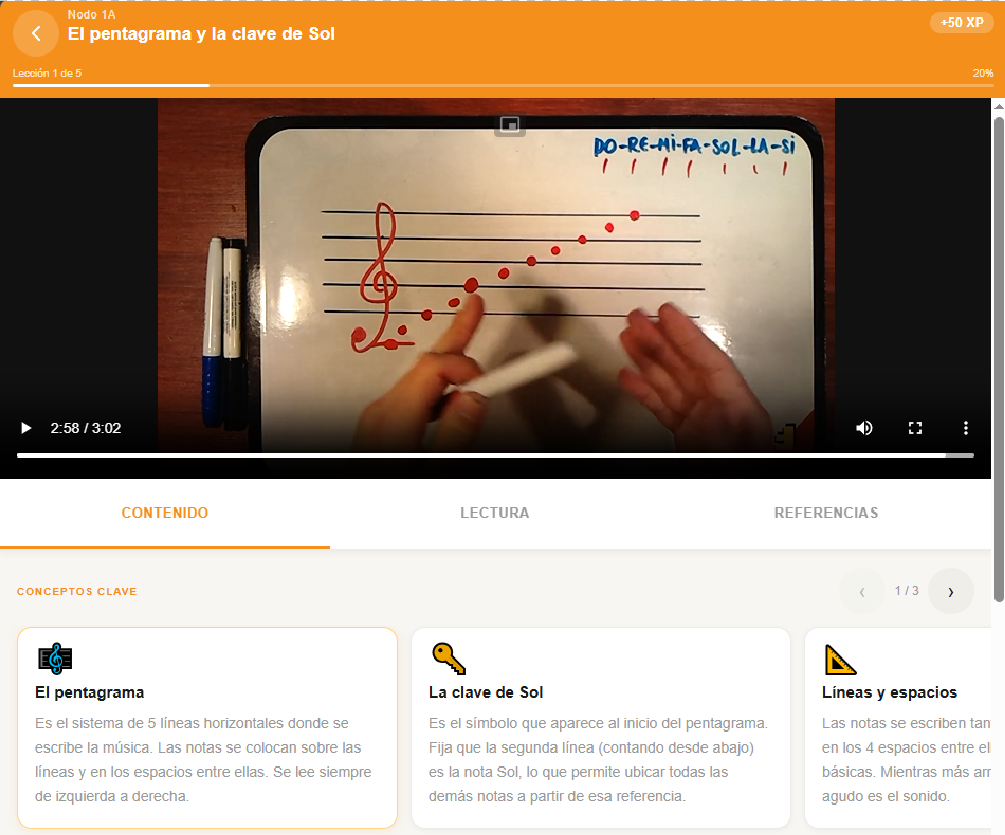
\includegraphics[width=0.3\textwidth]{Imagenes/MaterialAprendizajeFrontend.png}
    \caption{Renderizado dinámico del contenido pedagógico utilizando objetos JSONB recuperados desde el backend.}
    \label{fig:contenido}
\end{figure}

Una vez finalizada una actividad, se inicia el segundo flujo de interacción, correspondiente al proceso de recomendación adaptativa. Como se observa en la Figura~\ref{fig:inferencia}, el cliente envía el resultado del ejercicio al backend, el cual valida la sesión del usuario, actualiza el historial académico y construye el vector de observaciones requerido por el agente DRL. Posteriormente, el microservicio de inteligencia ejecuta el modelo PPO, determina la siguiente recomendación considerando el estado del estudiante y las restricciones impuestas por el Grafo de Conocimiento Musical, y retorna la respuesta al backend. Finalmente, la plataforma presenta al estudiante el siguiente ejercicio junto con su nivel de dificultad adaptativo, completando el ciclo de aprendizaje.

%--------------------------------------------------------
% FIGURA 5
%--------------------------------------------------------

\begin{figure}[htbp]
    \centering
    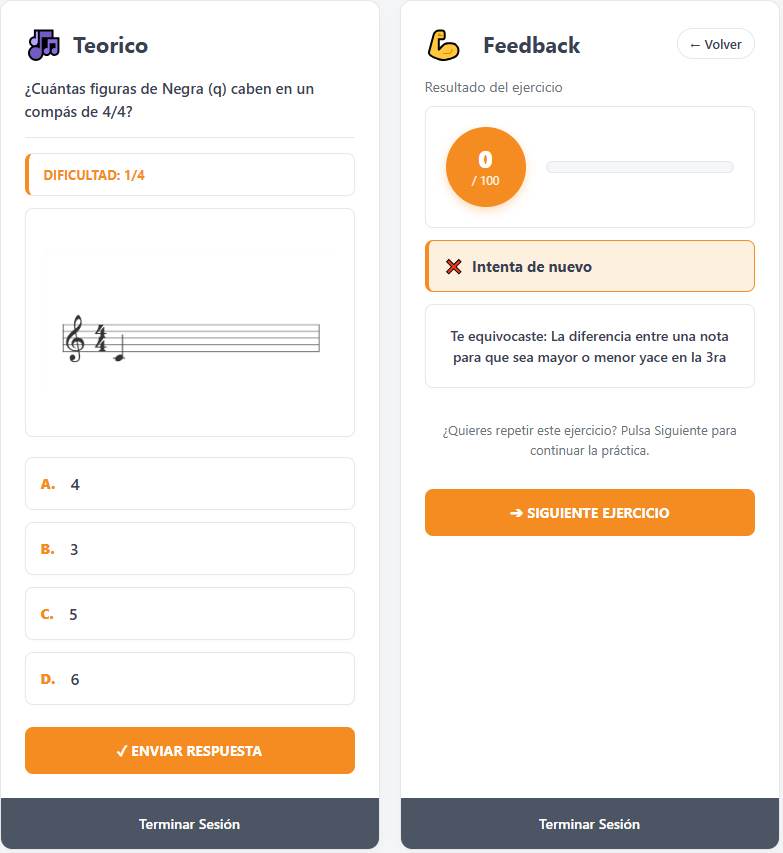
\includegraphics[width=0.3\textwidth]{Imagenes/frontend_ejercicio.png}
    \caption{Flujo distribuido de inferencia entre el cliente, el backend y el motor de Deep Reinforcement Learning.}
    \label{fig:inferencia}
\end{figure}

La arquitectura distribuida propuesta desacopla completamente la representación del conocimiento (DAG), el proceso de toma de decisiones basado en Deep Reinforcement Learning y la interfaz utilizada por estudiantes y docentes. Como consecuencia, nuevas estrategias de recomendación, funciones de recompensa o modelos de aprendizaje pueden incorporarse al sistema sin modificar la plataforma cliente, favoreciendo la mantenibilidad, escalabilidad y evolución futura de \textbf{SheetMusic}.

%\section{Arquitectura General del Sistema}
El sistema adopta el paradigma de arquitectura de microservicios distribuidos, separando la lógica de presentación, la capa de persistencia/autorización y el cómputo intensivo de Inteligencia Artificial. Esta separación garantiza escalabilidad horizontal y alta disponibilidad frente a concurrencia estudiantil \cite{charland_mobile_2011, flutter_vs_ionic_2023}.

\subsection{Capa de Cliente (Frontend - SheetMusic Pedia)}
Desarrollada con Ionic React v8 y Capacitor v7, empaquetada como Progressive Web App (PWA) e instalable de forma nativa en dispositivos móviles. Utiliza React Query para la gestión del estado remoto y emite peticiones HTTPS/RESTful autenticadas mediante tokens JSON Web Tokens (JWT).

\subsection{Capa de Servicios de Backend (BaaS)}
Se utiliza Supabase sobre PostgreSQL 15, desplegado en la región AWS \textit{us-east-1} \cite{supabase_docs_2024}. Esta capa administra la identidad de los usuarios, almacena el historial de progreso y la telemetría académica, y aplica políticas de Row Level Security (RLS) para aislar la información entre roles (estudiantes y docentes). Toda comunicación con el cliente se realiza a través de procedimientos almacenados remotos (RPC) para minimizar los viajes de ida y vuelta a la red (\textit{round trips}).

\subsection{Capa de Inteligencia (Motor DRL)}
Construido sobre FastAPI, PyTorch y Stable-Baselines3 en Debian/Docker. Recibe el vector de estado del estudiante desde la API REST de backend, procesa las restricciones pedagógicas del árbol y devuelve en milisegundos la recomendación del siguiente ejercicio junto a su nivel de dificultad.

\begin{figure}[htbp]
\centerline{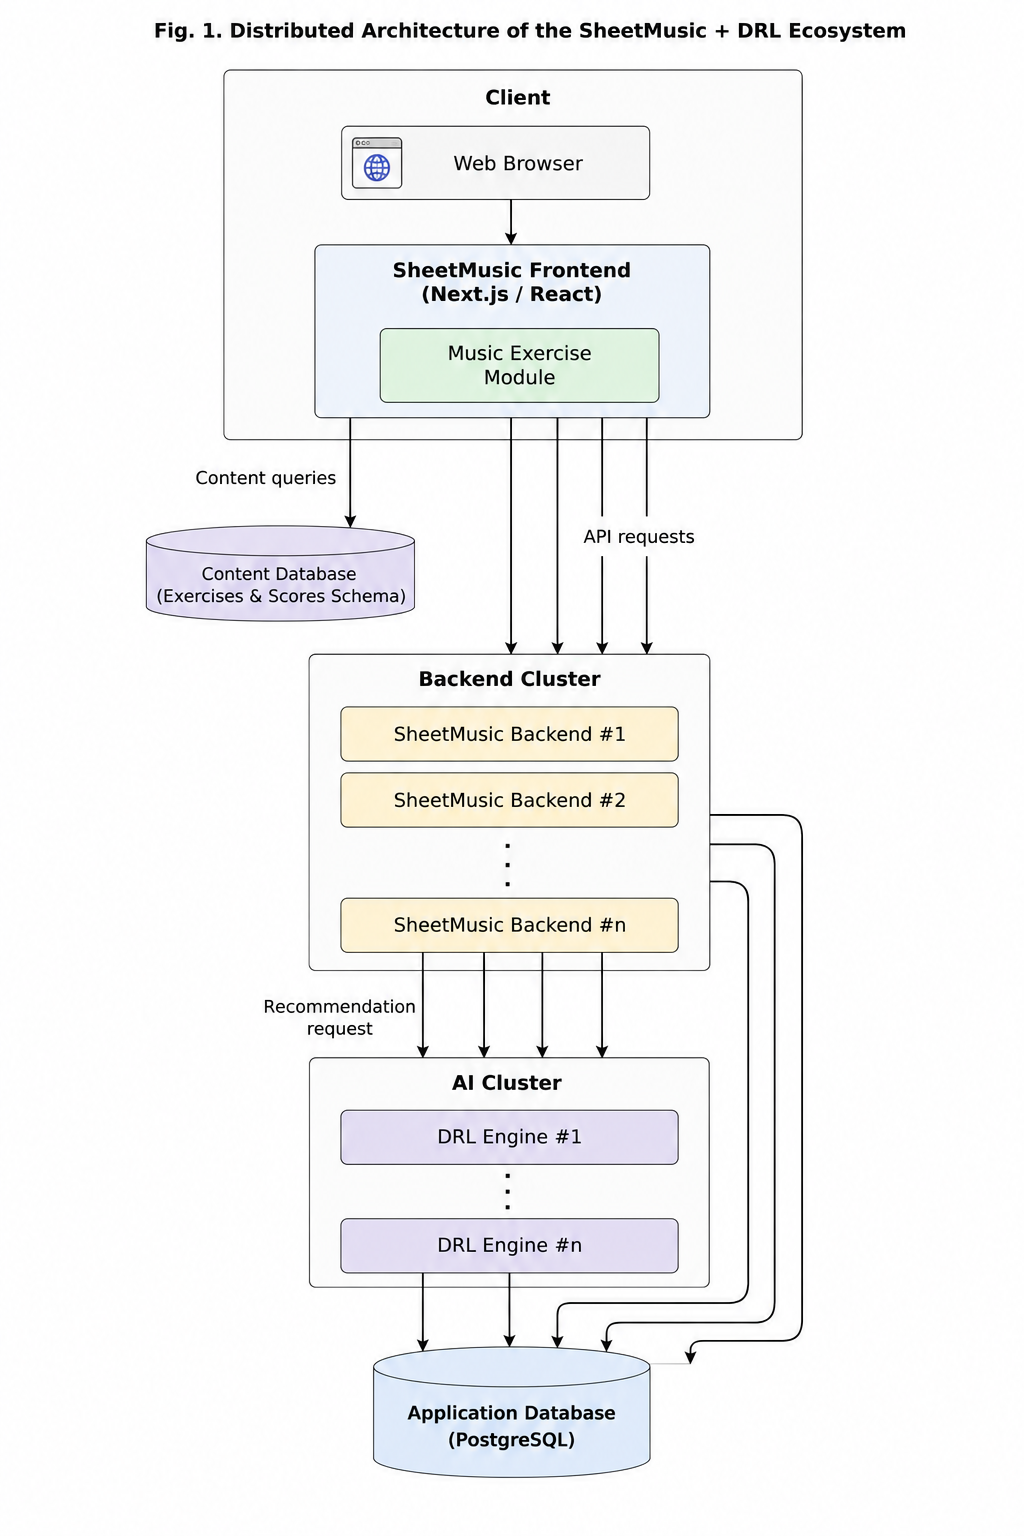
\includegraphics[width=0.48\textwidth]{Imagenes/fig_arch_system.png}}
\caption{Diagrama de arquitectura distribuida del ecosistema SheetMusic + DRL.}
\label{fig_arch}
\end{figure}

%\section{Modelo de Conocimiento, Árbol DAG y Gestión Pedagógica}

\subsection{Estructura Jerárquica del Grafo Dirigido Acíclico (DAG)}
El dominio de la teoría musical se formalizó mediante un Grafo Dirigido Acíclico (DAG) definido como $G = (V, E)$, donde $V$ representa el conjunto de 23 unidades de conocimiento (nodos) y $E$ corresponde a 29 aristas que codifican dependencias de prerrequisitos pedagógicos estrictos, fundamentado en la teoría de aprendizaje acumulativo de Gagné \cite{gagne_conditions_1985}. 

Los nodos se distribuyen en cinco bandas de dificultad identificadas por color:
\begin{itemize}
    \item \textbf{Nivel 1 (Iniciación - Gris):} Notas y Ritmo (1a), Entonación Simple (1b). Recompensa: 50 XP.
    \item \textbf{Nivel 2 (Fundamentos - Verde):} Intervalos (2a), Escalas (2b), Solfeo a dos voces (2c). Recompensa: 80 XP.
    \item \textbf{Nivel 3 (Armonía - Azul):} Acordes Tríadas (3a), Progresiones Básicas (3b), Dictado Melódico (3c). Recompensa: 120 XP.
    \item \textbf{Nivel 4 (Teoría Avanzada - Morado):} Acordes con Séptima (4a), Cadencias (4b), Dictado Armónico (4c). Recompensa: 160 XP.
    \item \textbf{Nivel 5 (Maestría - Dorado):} Contrapunto (5a), Armonía Cromática (5b), Análisis Complejo (5c). Recompensa: 200 XP.
\end{itemize}

\subsection{Algoritmo de Cálculo de Estado de Nodos y Modo Foco}
Para determinar la disponibilidad de un nodo en la interfaz web, el \textit{hook} \texttt{useSkillTreeData} recupera el grafo e invoca un algoritmo de ordenamiento topológico local. Un nodo $v_i \in V$ se clasifica dinámicamente según la regla:

\begin{equation}
State(v_i) = \begin{cases} 
\text{locked}, & \exists u \in Pred(v_i) \mid Prog(u) \neq \text{done} \\
\text{done}, & Prog(v_i) = \text{done} \\
\text{active}, & Prog(v_i) = \text{in\_progress} \\
\text{available}, & \text{en otro caso}
\end{cases}
\label{eq_state}
\end{equation}

El lienzo SVG dibuja los nodos mediante un algoritmo de disposición bidimensional por niveles y conecta las dependencias con curvas de Bézier cúbicas. La interfaz soporta un \textbf{Modo de Foco} (\textit{Focus Mode}) que, ejecutando un recorrido en amplitud (BFS) hacia atrás desde un nodo objetivo, aísla y resalta la ruta crítica de aprendizaje atenuando los nodos irrelevantes.

\subsection{Entrega Segura de Video y Motor de Gamificación en BD}
Para proteger los videos pedagógicos alojados en Supabase Storage, el cliente invoca la RPC \texttt{get\_signed\_url} \cite{aws_presigned_2023, owasp_mobile_2023}. Tras validar que el usuario ha desbloqueado el nodo, se genera una URL pre-firmada con 10 minutos de vigencia. El \textit{hook} \texttt{useVideoUrl} monitorea la expiración y solicita una nueva clave 2 minutos antes del vencimiento sin interrumpir la reproducción en curso.

La lógica de gamificación reside 100\% en la base de datos a través de \textit{triggers} transaccionales \cite{deterding_game_2011, hamari_does_2014}:
\begin{itemize}
    \item \texttt{trg\_xp\_leccion\_completada}: Acredita el valor \texttt{xp\_reward} con guardas de idempotencia.
    \item \texttt{trg\_xp\_cuestionario}: Otorga 80 XP base y un bono de 40 XP si se aprueba en el primer intento.
    \item \texttt{trg\_racha\_diaria}: Suma bonos de 100, 300 y 1000 XP al alcanzar rachas de 7, 30 y 100 días consecutivos de práctica.
\end{itemize}
El nivel del usuario se calcula automáticamente mediante la progresión geométrica $XP_{\min}(n) = 500 \times 2^{n-2}$ para $n \ge 2$.

\subsection{Panel de Gestión y Seguimiento Docente}
El módulo para el profesorado permite crear cursos, generar códigos alfanuméricos de inscripción y asignar tareas acotadas a un nodo completo o lección individual. A través de la RPC \texttt{get\_metricas\_leccion}, el docente visualiza la tasa de éxito porcentual de cada alumno, la cantidad de intentos fallidos acumulados y gráficos consolidados de actividad diaria del curso junto con las lecciones de mayor dificultad promedio.

%\section{Fundamentos del Motor de Deep Reinforcement Learning}

El motor de recomendación basado en Deep Reinforcement Learning (DRL) constituye el núcleo inteligente del sistema de enseñanza musical adaptativa. Su función principal es seleccionar el ejercicio más apropiado para cada estudiante en función de su estado de conocimiento actual, maximizando una función de recompensa que combina el acierto, la dificultad óptima y el tiempo de respuesta. La arquitectura se implementó siguiendo el patrón \textit{agent-environment loop} de Reinforcement Learning, utilizando \textit{Stable-Baselines3} (versión 2.0.1) y \textit{Gymnasium} (versión 1.2.0).

\subsection{Modelado del Conocimiento Musical}

El conocimiento musical fue modelado como un grafo dirigido etiquetado $G = (V, E)$, donde $V$ representa unidades de conocimiento (conceptos musicales) y $E$ representa relaciones de dependencia pedagógica no estrictas (\textit{soft prerequisite graph}). A diferencia de un grafo de prerrequisitos rígido, estas relaciones reflejan una estructura de aprendizaje preferencial donde ciertos conceptos facilitan la adquisición de otros, permitiendo flexibilidad en la progresión. Para acotar el espacio de estados del agente DRL, se implementó un subconjunto de cuatro nodos fundamentales: notas y ritmo, intervalos, escalas mayores y menores, y acordes tríadas. Este modelo fue validado con docentes del Conservatorio de Música de la Universidad Austral de Chile y de la Casona Cultural de Panguipulli.

\subsection{Arquitectura del Entorno de Aprendizaje (MusicLearningEnv)}

El entorno \texttt{MusicLearningEnv} se implementó como subclase de \texttt{gymnasium.Env}, modelando la interacción agente-estudiante donde cada paso corresponde a seleccionar un ejercicio y recibir retroalimentación.

\subsubsection{Espacio de Observaciones}

El estado se representa mediante la clase \texttt{UserState}, que encapsula: \textbf{knowledge} (proficiencia $[0.0, 1.0]$ por nodo), \textbf{accuracy} (precisión histórica), \textbf{attempts} (intentos por nodo), \textbf{streak} (racha de aciertos/fallos), \textbf{last\_exercise\_difficulty} (dificultad escala 1--10), \textbf{time\_since\_last\_practice} (horas desde última práctica) y \textbf{recent\_performance\_trend} (últimos 10 resultados por nodo). Para inferencia, el estado se binariza con umbral 0.5:
\begin{equation}
o_i = \begin{cases} 
1 & \text{si } \text{proficiency}_i \geq 0.5 \\
0 & \text{en otro caso}
\end{cases}
\end{equation}
resultando en un vector \texttt{MultiBinary(N)} con $N$ nodos activos.

\subsubsection{Espacio de Acciones}

Espacio discreto \texttt{Discrete(N)} donde cada acción es un índice mapeado a un ejercicio mediante \texttt{skill\_mapping}. Esto permite agregar o eliminar nodos sin reentrenar el modelo, y garantiza que toda acción corresponda a un ejercicio válido.

\subsubsection{Función de Recompensa}

Combina múltiples factores para balancear consolidación y exploración:
\begin{equation}
\begin{aligned}
R =\;&
1.0\,\mathbb{I}(\text{correcto})
+ 0.5\,\mathbb{I}(\text{mejoría}) \\
&+ 0.5\,\mathbb{I}\!\left(
    \left| d - d^{*} \right| \leq 1
\right)
- 0.3\,\mathbb{I}\!\left(
    \left| d - d^{*} \right| > 2
\right) \\
&+ 0.2\,\mathbb{I}(\text{nodo poco practicado})
+ 0.1\,\mathbb{I}(\text{ejercicio nuevo})
\end{aligned}
\end{equation}

Los términos incentivan: (1) acierto, (2) mejora respecto al intento anterior, (3) dificultad en zona de desarrollo proximal ($d^* = \text{proficiency} \times 10$), (4) penalización por dificultad inadecuada, (5) exploración de nodos con $<3$ intentos, y (6) variedad de ejercicios. Adicionalmente, se penaliza con $-1.0$ si no se cumplen prerrequisitos (proficiencia $>0.6$ en nodos previos) y con $-0.5$ la repetición consecutiva del mismo ejercicio.

\subsection{Selección del Algoritmo: DQN vs PPO}

Se evaluaron dos algoritmos. \textbf{DQN} (\textit{value-based}) mostró convergencia rápida inicial ($\approx$120 episodios para recompensa 0.75), pero tendió a políticas conservadoras que evitaban nodos nuevos por sobreestimación de valores Q. \textbf{PPO} (\textit{policy-based}, actor-critic) con arquitectura MLP de dos capas ocultas de 64 unidades, clipping $\epsilon=0.2$ y learning rate $3\times10^{-4}$, mostró convergencia más lenta inicialmente (150--180 episodios) pero desarrolló políticas más estables y balanceadas entre exploración y explotación. Se seleccionó PPO por su estabilidad, manejo de incertidumbre educativa, facilidad de ajuste, políticas estocásticas (evitan patrones predecibles) y despliegue simplificado al no requerir replay buffer.

\subsection{Generación de Experiencias de Entrenamiento Basadas en Encuestas}

Dado que en fases iniciales no se disponía de datos reales de interacción, se diseñó un proceso de generación de experiencias en dos etapas. Primero, se aplicó un cuestionario mediante \textbf{Google Forms} a estudiantes de enseñanza media para estimar distribuciones de comportamiento, niveles de conocimiento inicial y parámetros del modelo de aprendizaje. Segundo, a partir de estos parámetros empíricos, se implementó un simulador probabilístico (\texttt{SyntheticStudent}) que genera trayectorias de entrenamiento realistas.

Se definieron tres perfiles basados en los datos de las encuestas: \textbf{desde\_cero} (proficiencias 0.1--0.35 en nodos básicos), \textbf{parcial} (dominio intermedio 0.5--0.8 en nodos avanzados) y \textbf{avanzado} (dominio alto 0.6--0.9). El modelo \texttt{SyntheticStudent} incluye tasa de aprendizaje individual (factor 0.9--1.4), umbral de frustración, consistencia de habilidad y nodos dominados. La actualización tras cada interacción sigue: en éxito, incremento de proficiencia proporcional a la tasa de aprendizaje (máx. 0.3); en fallo, penalización $0.15 \times (1 - \text{consistencia}) + 0.1 \times (\text{fallos previos} + 1)$.

El entrenamiento se realizó en dos etapas: \textbf{Behavior Cloning} inicial (red fully-connected de 128 unidades, entropía cruzada, Adam con $10^{-3}$, 5 épocas) para establecer una política base, seguido de \textbf{entrenamiento PPO} (10,000 pasos, política MlpPolicy, CPU). El dataset generó aproximadamente 150,000--200,000 pasos de entrenamiento.

\subsection{API de Inferencia y Validación Experimental}

El modelo se expone mediante \texttt{FastAPI} con dos endpoints principales: \texttt{POST /next-exercise} (recibe el estado del estudiante y retorna la recomendación PPO con dificultad adaptativa) y \texttt{POST /session-end} (calcula recompensa de sesión y actualiza proficiencias). El modelo se carga con \textit{lazy loading} thread-safe.

La validación se realizó con 28 estudiantes (5 del Conservatorio de la UACh, 23 de enseñanza media de Corral) durante 28 días. Se analizaron tres perfiles de rendimiento: mejor, promedio y menor estudiante. Los resultados mostraron una mejora mediana del 20\% en \textit{proficiency}, superando el objetivo del 15\%, y la actividad se mantuvo sostenida durante las cuatro semanas. Dado que la validación correspondió a un piloto de un solo grupo, sin grupo control ni pruebas de significancia, estos resultados constituyen evidencia preliminar de factibilidad y no permiten atribuir la mejora observada específicamente al motor DRL.
\section{VALIDACIÓN EXPERIMENTAL}

Con el objetivo de validar la propuesta presentada, se diseñó una evaluación que consideró tanto el desempeño del modelo de aprendizaje adaptativo como la percepción de los usuarios respecto de la plataforma \textbf{SheetMusic}. La validación se estructuró en tres etapas: (i) definición del escenario experimental, (ii) evaluación mediante métricas objetivas y subjetivas, y (iii) análisis de los resultados obtenidos.

%--------------------------------------------------------
\subsection{Diseño Experimental}

La validación se realizó utilizando la versión funcional de \textbf{SheetMusic} desarrollada durante el proyecto. Los participantes interactuaron con la plataforma resolviendo actividades de teoría musical recomendadas por el agente basado en \textit{Deep Reinforcement Learning}. Durante cada sesión se registró automáticamente el estado del estudiante, las recomendaciones realizadas por el sistema y el progreso alcanzado en las distintas unidades de conocimiento.

Finalizada la interacción, estudiantes y docentes respondieron instrumentos estandarizados con el propósito de evaluar la usabilidad y aceptación de la plataforma.

%--------------------------------------------------------
\subsection{Métricas de Evaluación}

La validación experimental consideró dos dimensiones complementarias: (i) el desempeño del modelo de recomendación basado en \textit{Deep Reinforcement Learning} y (ii) la percepción de los usuarios respecto de la plataforma \textbf{SheetMusic}.

\textbf{Evaluación del modelo de recomendación.} Para analizar el comportamiento del agente DRL se utilizaron los siguientes indicadores:

\begin{itemize}

\item \textbf{Progreso de Aprendizaje (Proficiency):} cuantifica el incremento del nivel de dominio alcanzado por el estudiante durante las sesiones de aprendizaje, permitiendo evaluar la efectividad pedagógica de las recomendaciones generadas por el agente.

\item \textbf{Tasa de Continuidad:} mide la permanencia del estudiante en el proceso de aprendizaje mediante el número de sesiones realizadas y la continuidad de uso de la plataforma, proporcionando una estimación indirecta del nivel de compromiso generado por el sistema adaptativo.

\item \textbf{Adaptabilidad de la Dificultad:} evalúa la capacidad del agente para recomendar ejercicios cuya dificultad se mantenga cercana al nivel de competencia del estudiante, evitando tanto la frustración por actividades excesivamente complejas como la pérdida de interés por ejercicios demasiado simples.

\end{itemize}

\textbf{Evaluación de la plataforma.} Para analizar la experiencia de uso de \textbf{SheetMusic} se emplearon instrumentos ampliamente utilizados en la evaluación de sistemas interactivos:

\begin{itemize}

\item \textbf{Usabilidad (SUS):} se aplicó el cuestionario \textit{System Usability Scale (SUS)} para evaluar la facilidad de uso percibida por los estudiantes~\cite{sus_brooke_1996}.

\item \textbf{Aceptación Tecnológica (TAM):} los docentes respondieron un cuestionario basado en el \textit{Technology Acceptance Model (TAM)}, permitiendo evaluar la utilidad percibida, la facilidad de uso y la intención de utilización futura de la plataforma~\cite{davis1989}.

\end{itemize}

%--------------------------------------------------------
\section{RESULTADOS}

%--------------------------------------------------------
\subsection{Resultados}

La validación experimental se realizó mediante una prueba piloto con 28 estudiantes de la Región de Los Ríos, Chile, compuesta por 5 estudiantes del Conservatorio de Música de la Universidad Austral de Chile y 23 estudiantes de enseñanza media de la comuna de Corral. Durante un período de 28 días consecutivos, los participantes utilizaron la plataforma \textbf{SheetMusic} para resolver actividades de teoría musical recomendadas por el agente basado en \textit{Deep Reinforcement Learning}, registrándose automáticamente las métricas de interacción, progreso y rendimiento utilizadas en la evaluación.

%--------------------------------------------------------
\subsubsection{Resultados del Modelo de Recomendación}

La Figura~\ref{fig:rendimiento_ieee} presenta la evolución del nivel de \textit{proficiency} para tres perfiles representativos de estudiantes: alto, medio y bajo desempeño. En los tres casos se observa una tendencia ascendente, indicando que el agente fue capaz de adaptar progresivamente las recomendaciones al nivel de conocimiento de cada estudiante. Incluso los participantes con menor dominio inicial evidenciaron una mejora sostenida durante el período de evaluación, lo que sugiere que la política aprendida mediante PPO logra personalizar adecuadamente las trayectorias de aprendizaje.

\begin{figure}[htbp]
    \centering
    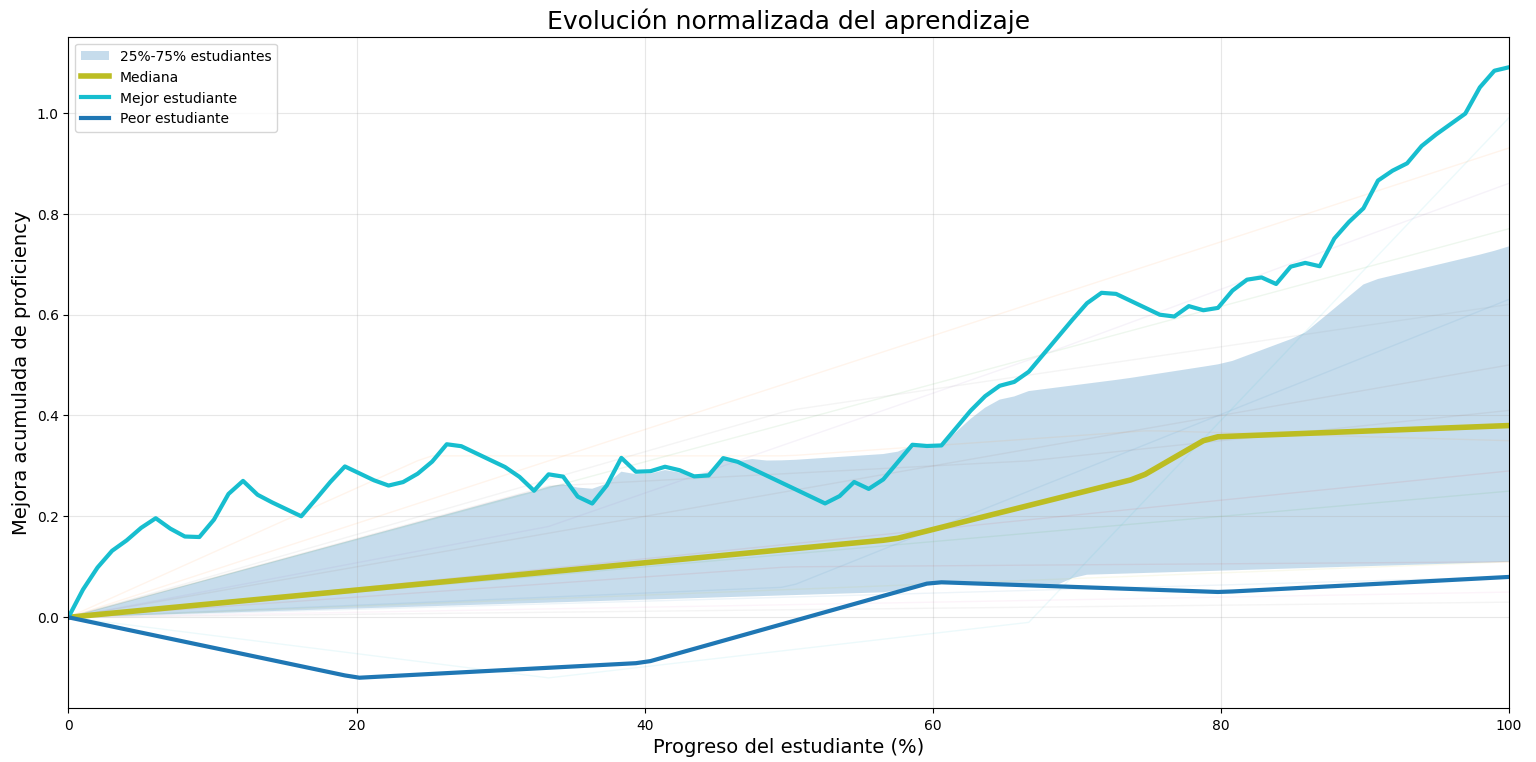
\includegraphics[width=0.48\textwidth]{Imagenes/rendimiento_estudiantes.png}
    \caption{Evolución del nivel de \textit{proficiency} de tres perfiles representativos de estudiantes durante la validación experimental.}
    \label{fig:rendimiento_ieee}
\end{figure}

La continuidad de uso fue evaluada mediante el número de sesiones registradas durante el período experimental. Como se observa en la Figura~\ref{fig:actividad_ieee}, la actividad se mantuvo estable durante las tres primeras semanas de evaluación, acumulando un total de 572 sesiones. La disminución observada durante la cuarta semana corresponde al cierre del proceso de recolección de datos y no a una disminución en el uso de la plataforma.

\begin{figure}[htbp]
    \centering
    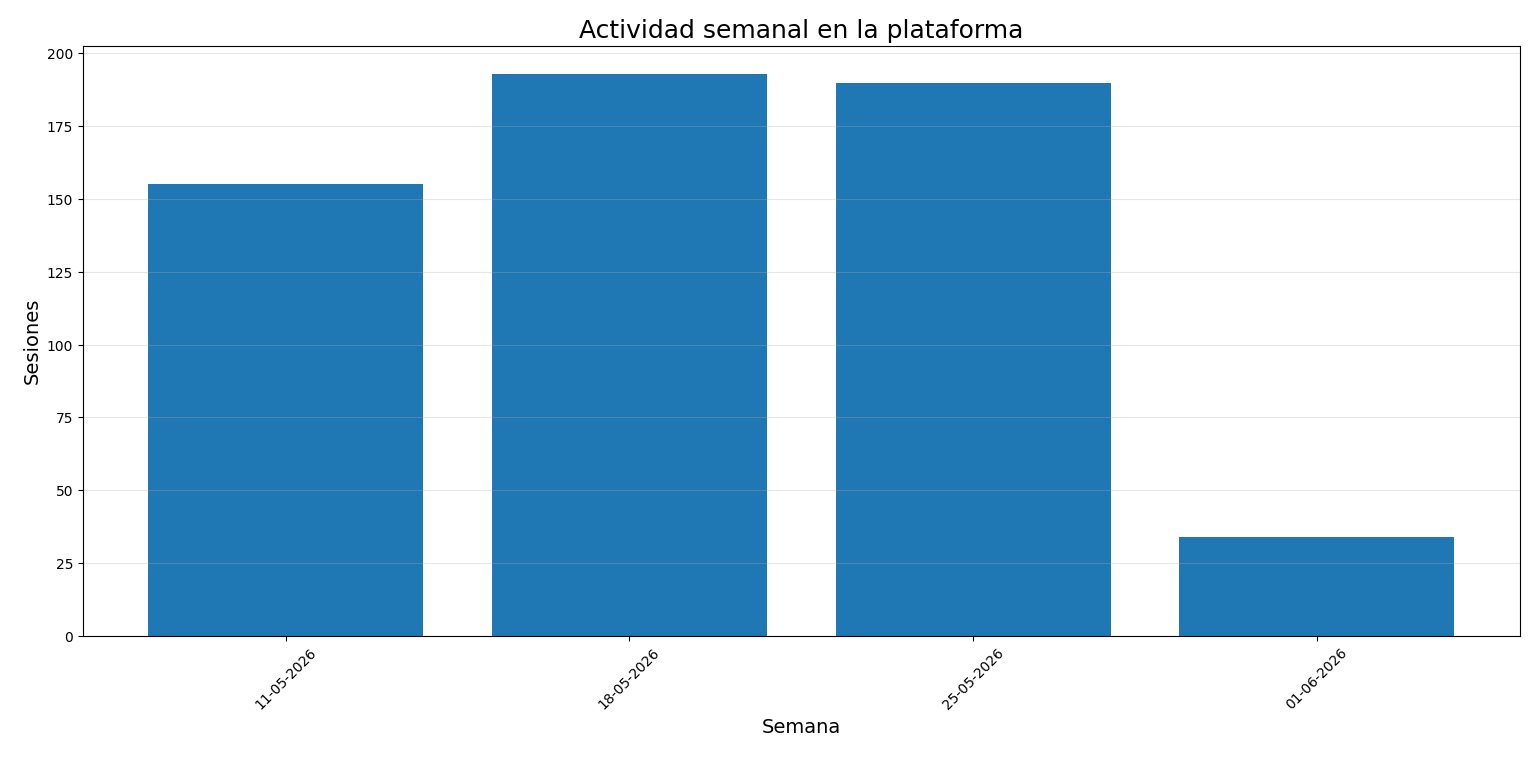
\includegraphics[width=0.48\textwidth]{Imagenes/actividad_semanal.png}
    \caption{Distribución semanal de las sesiones registradas durante el período de validación.}
    \label{fig:actividad_ieee}
\end{figure}

Los principales indicadores obtenidos durante la validación se resumen en la Tabla~\ref{tab:resultados_ieee}. En particular, la mediana del nivel de \textit{proficiency} presentó una mejora aproximada del 20\%, superando la meta inicial del 15\%. Asimismo, el sistema ajustó dinámicamente la dificultad y la secuencia de ejercicios de acuerdo con el desempeño individual de cada estudiante, evidenciando la capacidad del agente DRL para personalizar el proceso de aprendizaje.

\begin{table}[htbp]
\centering
\caption{Resumen de los principales resultados obtenidos durante la validación del modelo de recomendación.}
\label{tab:resultados_ieee}
\begin{tabular}{lp{5.2cm}}
\hline
\textbf{Indicador} & \textbf{Resultado} \\
\hline
Participantes & 28 estudiantes \\
Sesiones registradas & 572 sesiones \\
Continuidad de uso & Actividad sostenida durante el período de evaluación \\
Mejora en \textit{Proficiency} & Incremento aproximado del 20\% (meta: 15\%) \\
Adaptabilidad & Ajuste dinámico de la dificultad y secuencia de ejercicios según el desempeño del estudiante \\
\hline
\end{tabular}
\end{table}

En conjunto, estos resultados indican que el agente basado en \textit{Deep Reinforcement Learning} fue capaz de mantener una progresión positiva del aprendizaje, adaptar las recomendaciones al desempeño individual de los estudiantes y sostener una participación continua durante el período de evaluación.

%--------------------------------------------------------
\subsubsection{Resultados de la Plataforma}

La plataforma \textbf{SheetMusic} fue evaluada desde la perspectiva de la experiencia de usuario utilizando los instrumentos \textit{System Usability Scale} (SUS) y \textit{Technology Acceptance Model} (TAM). Los resultados obtenidos se resumen en la Tabla~\ref{tab:sus_tam}.

\begin{table}[htbp]
\centering
\caption{Resultados de la evaluación de usabilidad y aceptación tecnológica de la plataforma.}
\label{tab:sus_tam}
\begin{tabular}{lc}
\hline
\textbf{Métrica} & \textbf{Resultado} \\
\hline
System Usability Scale (SUS) & 82.5 / 100 \\
Future Use Perception (FUP) & 4.00 / 5.00 \\
\hline
\end{tabular}
\end{table}

El puntaje obtenido en SUS indica una percepción positiva respecto de la facilidad de uso de la plataforma, mientras que la evaluación de Future Use Perception evidencia una favorable disposición de los participantes a continuar utilizando la herramienta en futuros procesos de enseñanza y aprendizaje. En conjunto, estos resultados complementan la evaluación técnica del modelo de recomendación, mostrando que la propuesta no sólo adapta el proceso de aprendizaje, sino que además presenta un nivel de usabilidad y aceptación adecuado para su utilización en contextos educativos.
\section{CONCLUSIONES Y TRABAJOS FUTUROS}

En este trabajo se presentó un modelo computacional de aprendizaje adaptativo para la enseñanza de teoría musical, el cual integra un Grafo de Conocimiento Dirigido Acíclico (DAG) para representar explícitamente las dependencias pedagógicas del dominio y un agente basado en \textit{Deep Reinforcement Learning} para recomendar dinámicamente actividades de aprendizaje de acuerdo con el progreso individual del estudiante. El modelo fue implementado mediante la plataforma distribuida \textbf{SheetMusic}, permitiendo materializar la propuesta en un entorno real de apoyo al proceso de enseñanza y aprendizaje.

Los resultados de la validación experimental muestran que el agente de recomendación fue capaz de adaptar la secuencia y dificultad de los ejercicios según el desempeño de cada estudiante, favoreciendo una progresión sostenida del nivel de conocimiento y manteniendo una participación continua durante el período de evaluación. Asimismo, la evaluación de usabilidad y aceptación tecnológica evidenció una percepción favorable de la plataforma por parte de sus usuarios, respaldando la viabilidad de la propuesta para su utilización en contextos educativos.

Desde la perspectiva de la Ingeniería Informática, uno de los principales aportes del trabajo corresponde a la integración de una representación explícita del conocimiento pedagógico mediante un DAG con un modelo de aprendizaje por refuerzo profundo, desacoplando la estructura del dominio, el proceso de toma de decisiones y la implementación de la plataforma. Esta arquitectura facilita la evolución independiente de cada componente, permitiendo incorporar nuevos contenidos, estrategias de recomendación o modelos de inteligencia artificial sin modificar la infraestructura principal de \textbf{SheetMusic}.

Con el propósito de favorecer la reproducibilidad científica y la continuidad del proyecto, el código fuente de la plataforma, del motor de recomendación y de los microservicios desarrollados se encuentra disponible públicamente en la organización oficial de GitHub: \url{https://github.com/Sheetmusic-Team}.

Como trabajo futuro se contempla ampliar el Grafo de Conocimiento Musical para cubrir la totalidad de las unidades curriculares de teoría musical, incorporar nuevos modelos de aprendizaje por refuerzo y comparar su desempeño con PPO, integrar evaluación instrumental en tiempo real mediante procesamiento digital de señales (DSP) y validar la plataforma con una muestra significativamente mayor de estudiantes pertenecientes a distintos establecimientos educacionales del país.
\bibliographystyle{IEEEtran}
\bibliography{referencias}

\end{document}